\subsection{Period 3: Absence of DHL with sporadic transitory layers after the Northern Spring Equinox (2012-2015) - $L_s=\ang{30}-\ang{75}$}

During this period, the main haze layer has large scale structures which slowly evolve under the influence of the
large scale circulation. The south and north polarhoods are still visible and they evolve
with time. Superimposed to this background haze, transient structures show up and disappear from one observation
to the other. At some moments, large scale detached hazes appear. They differ from the detached haze seen at the
beginning of the mission because they are not stable in time and in altitude. They do not appear from one
observation to the other. The haze during this period is displayed in Fig.~\ref{fig:dhl_2012_2015}.

\begin{figure*}[!ht]
    \centering
    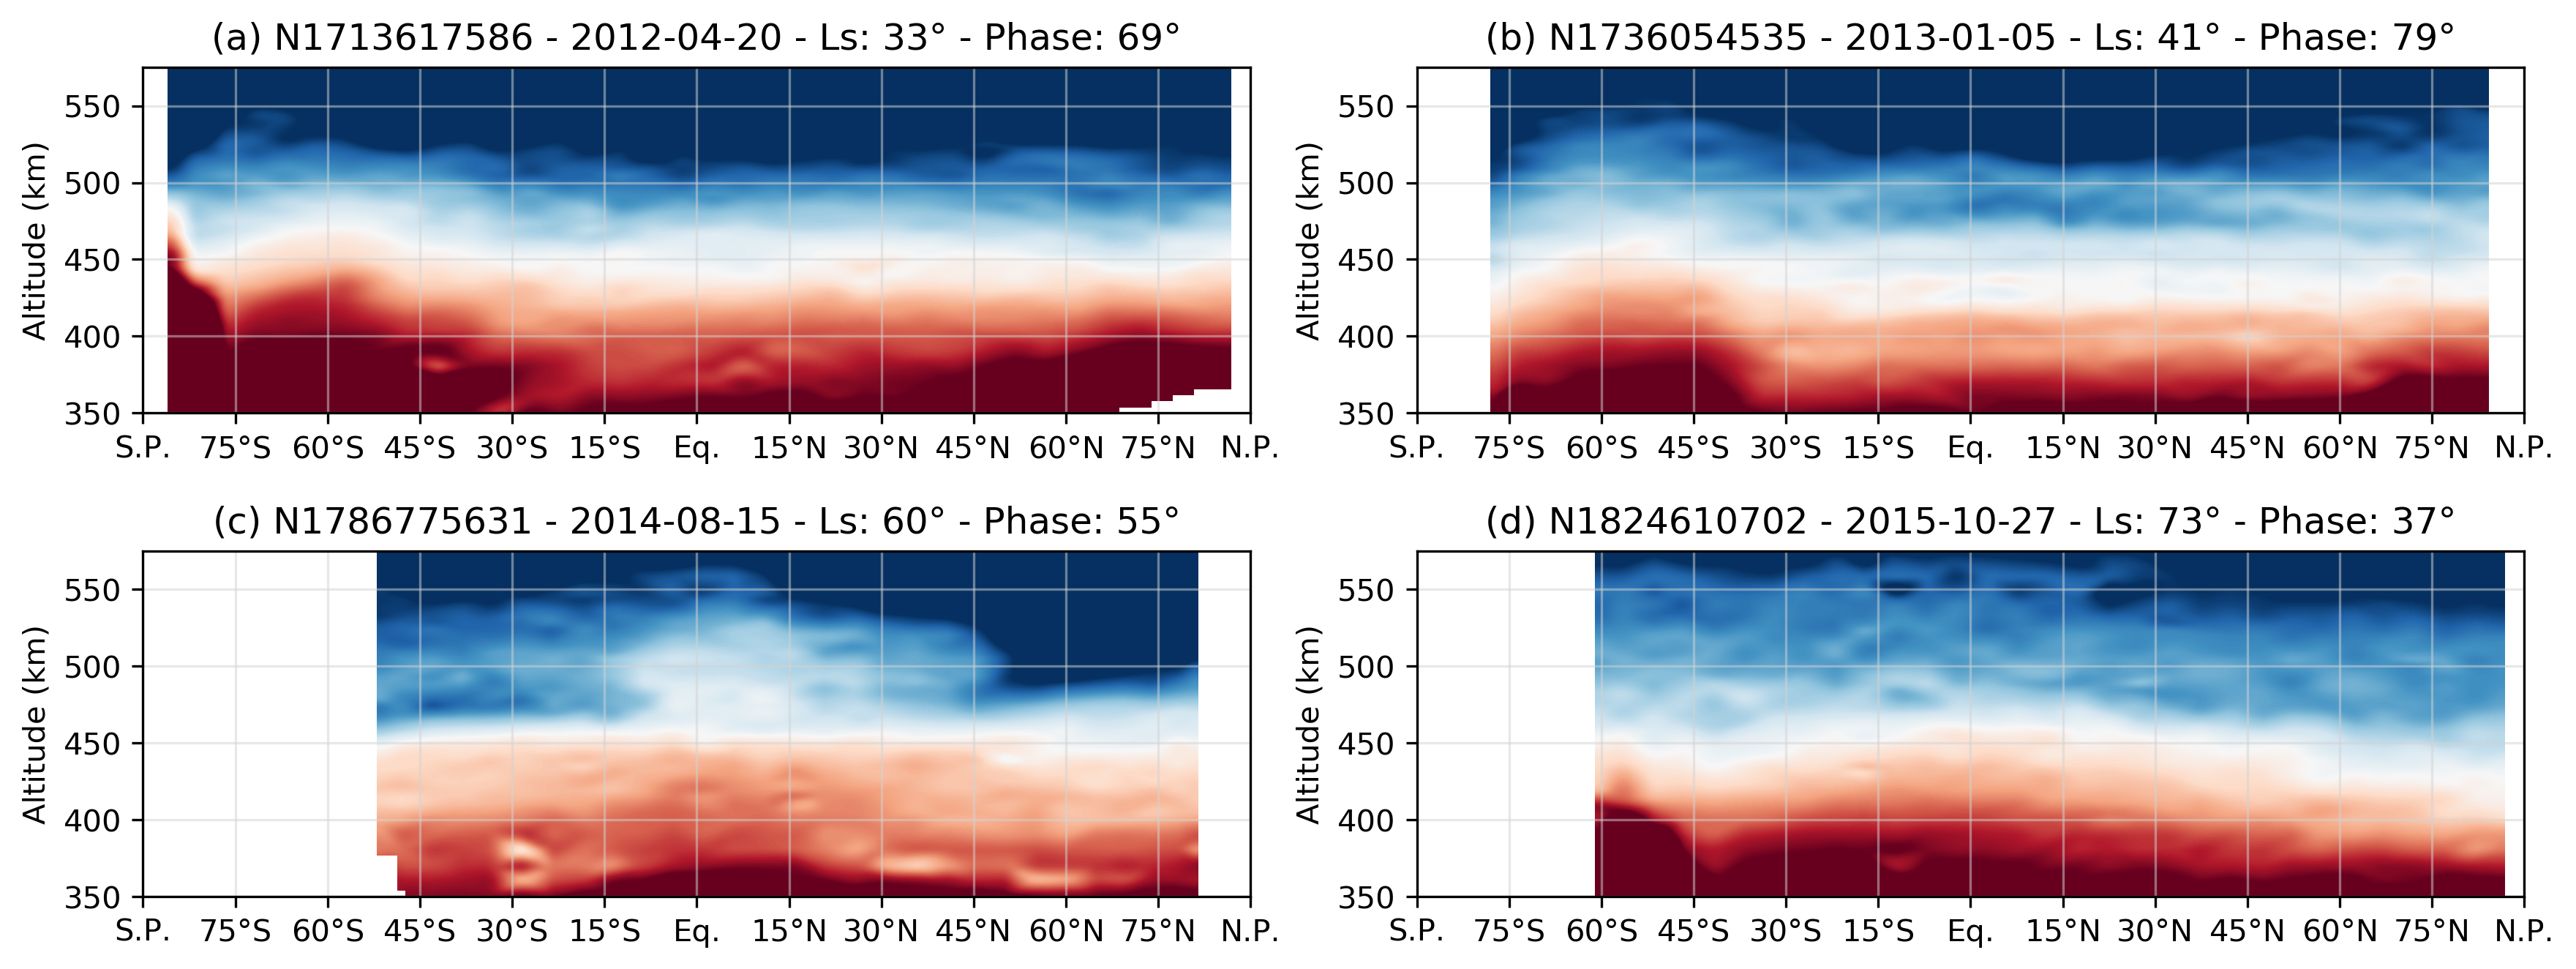
\includegraphics[width=\textwidth]{Fig/Lat_beta-2012_2015.png}
    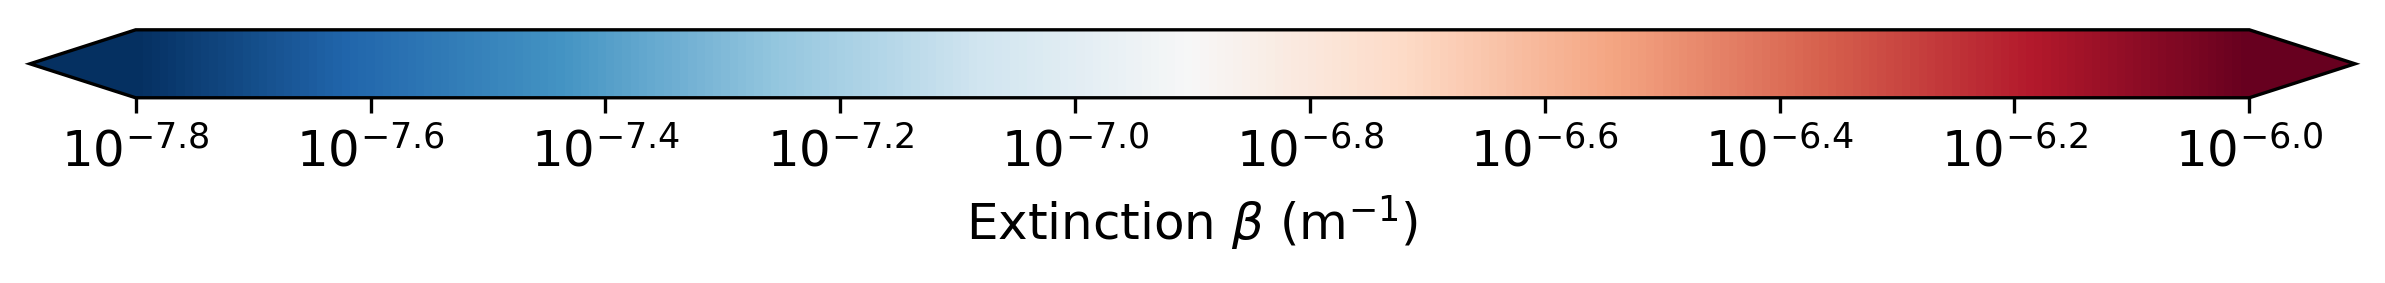
\includegraphics[width=.5\textwidth]{Fig/Extinction_colorbar.png}\vspace{-.3cm}
    \caption{Same as the figures~\ref{fig:dhl_2004_2008} and~\ref{fig:dhl_2008_2012}
    for 4 images taken between 2012 and 2015 ($L_s=\ang{30}-\ang{75}$) showing sporadic
    transitory layers and the absence of consistent DHL.
    The color extent is the same and the altitude ranges down to 350 km.}
    \label{fig:dhl_2012_2015}
\end{figure*}

In April 2012 (Fig.~\ref{fig:dhl_2012_2015}a), the detached haze has completely disappeared, except a residual
structure at \ang{5}-\ang{20}S, around 370 km.
This relict of the last detached haze layer is almost not perceptible in the corresponding I/F profile. At other
latitudes, we only can see a unique main haze with a marked south polarhood and a small increase of extinction above
\ang{65}N that could be the north polarhood. Sometimes, detached layers emerge from the background with large latitudinal
extent (e.g. detached haze at 500 km Fig.~\ref{fig:dhl_2012_2015}b). However, they only remain for a short time
and are not seen in the following observations.

In August 2014 (Fig.~\ref{fig:dhl_2012_2015}c) we observed a plume of aerosol between \ang{10}S and \ang{25}N,
at 500 km. A detached haze layer seems to have spread from this plume toward the north and the south. This
detached haze is around 500 km, descending to 470 km at \ang{60}S (and probably even southern). At the
north, the detached haze does not extend northern than \ang{50}N and remains at 500 km. This indicate an
atmosphere circulation rather flowing from equator toward the south pole. The origin of these aerosols is undefined.

The observation of October 2015 (Fig.~\ref{fig:dhl_2012_2015}d) is very representative of the haze layer in
the period between 2012 and the end of 2015. At this date, the main haze has a uniform scale height of 45 km and
with a homogenous extinction at the planetary scale.
